\section{Ejercicio 6}

\subsection{Introducción}
\noindent El objetivo de este ejercicio es resolver nuevamente el problema de MCS, pero esta vez con una metaheurística de búsqueda tabú, ya que suponemos que resolver el problema de forma exacta no se puede hacer en tiempo polinomial, pero sí podemos implementar un algoritmo heurístico que se ejecute eficientemente (tiempo polinomial) aunque no garantice la solución óptima.
\subsection{Metaheurística}
\noindent La búsqueda tabú es una metaheurística que al igual que búsqueda local busca pasar de una solución a otra e intenta corregir el problema del estancamiento en óptimos locales, es decir, que no se quede iterando siempre en una rama de soluciones cuando podría haber una solución mejor en otro lado. Para solucionar este problema, búsqueda tabú permite pasar de una solución a otra por más de que la segunda no sea mejor. Esto puede llevar a que el algoritmo se quede ciclando dentro de las mismas soluciones siempre. Por ejemplo, dado S óptimo local y S' mejor solución vecina de S y también S mejor solución vecina de S' pasaríamos de S a S' y luego de nuevo a S y así seguiríamos ciclando. Para solucionar esto se implementará una lista tabú la cual contendrá las últimas soluciones tomadas de forma que no pueda volver a repetirlas. Si sólo mantuviéramos la última solución podría pasar que el ciclo fuera entre 3 o más soluciones. Luego mencionaremos otras formas de implementar tabú search sin guardar soluciones enteras. Dejar muchas soluciones se basa en la idea de que al alejarse lo suficiente de una solución es muy poco probable que se vuelva a la misma. La cantidad de soluciones a dejar dentro de la lista tabú es un punto a analizar en este ejercicio. No sólo está el problema de la memoria que ocuparía guardar todas las soluciones ya visitadas si no que también al tener demasiadas soluciones guardadas, cada vez que se quiera mirar si una solución nueva posible se encuentra o no en la lista tabú se perdería muchísimo tiempo revisando una por una las soluciones que se encuentran guardadas y comparando con la nueva a ver si coincide. 

\subsubsection*{Vecindades}
\noindent En este ejercicio se analizarán dos criterios distintos para determinar cuando una solución es vecina de otra.
Las vecindades a utilizar son las mismas que las utilizadas en el ejercicio 5. 

\subsubsection*{Variaciones de búsqueda tabú}
\noindent Para la metaheurística de búsqueda tabú existen variaciones en diferentes aspectos del algoritmo. Por ejemplo, en la lista tabú se podrían guardar en lugar de soluciones ya visitadas, movimientos hechos para no repetirlos o características de las soluciones que no debería repetir. Otro de los aspectos que se pueden variar son los criterios de terminación, es decir, cuándo se considera que ya se iteró sobre la suficiente cantidad de vecinos y el resultado ya debería ser, en la mayoría de los casos, muy próximo a la solución real. Algunos ejemplos de los criterios que se pueden utilizar son:
\begin{itemize}
    \item No se encontró una mejora en las últimas k iteraciones.
	\item Se alcanzó un límite prefijado de k iteraciones.
	\item Se alcanzó un límite prefijado de tiempo.
    \item Se obtuvo una solución cercana a una cierta cota conocida.
    \item En las últimas k iteraciones todas las soluciones fueron tabú.
\end{itemize}
También se puede variar el tamaño de la lista tabú. Como ya mencionamos antes no solo está el problema de la memoria que ocupa si no que también al tener demasiadas soluciones guardadas cada vez que se quiera mirar si una solución nueva posible se encuentra o no en la lista tabú se deberá revisar una por una las soluciones que se encuentran guardadas y compararlas con la nueva a ver si coincide, lo que puede ser muy costoso. \\
Además, si algún mapeo tiene demasiados vecinos, mirar todos y decidir cual es el mejor también es muy costoso, por lo que la cantidad de vecinos de un mapeo que se tendrá en cuenta también es un criterio que puede variar. \\
En el algoritmo planteado para resolver este ejercicio el criterio de parada que se utilizó fue parar cuando no se haya encontrado una mejora en las últimas k iteraciones, donde k es un parámetro que se recibirá por parámetro al igual que el tamaño máximo que puede tener la lista tabú y la cantidad de vecinos de un mapeo que se tendrá en cuenta para determinar el mejor vecino.\\
La cantidad de vecinos a tener en cuenta debe ser mayor que el tamaño máximo que puede tener la lista tabú. De esta forma nos aseguramos que seguro al menos uno de ellos no se encontrará en la lista tabú. En caso de que la cantidad de vecinos totales que tiene la solución actual sea menor que la cantidad de vecinos a tener en cuenta y menor al tamaño máximo que puede tener la lista tabú, podría pasar que todos los vecinos estén en la lista tabú. Como es un caso muy particular asumimos que no va a suceder nunca.

\subsection{Implementación}
\noindent La lista tabú se usa en dos ocasiones, una para ver si algo está o no en la lista tabú, y otra para actualizarla (agregar soluciones, y si se llenó sacar la más vieja). En cada iteración la consulto para cada vecino y la actualizo una sola vez. Entonces, para poder consultar la lista de forma rápida para ver si una solución está o no en la lista, se utilizará $set<vector<int>> tabuPorMapeo$ que busca soluciones en $O(log cantSoluciones * tamano de las soluciones)$. En esta estructura, saber cuál fue el primero agregado, es decir, el mapeo que debo sacar cuando la lista tabú llega a su tamaño máximo y se quiere consultar por un nuevo vecino, es complicado. Por lo tanto se tendrá en paralelo con el set, la información también en un $queue<vector<int> >$ tabuCola, que es una cola fifo. Luego, comparar soluciones es preguntarle al set si la tiene.

 \begin{algoritmo}{MCSTabu}{vector(int) mapeo, vector(vector(int)) grafoChico, vector(vector(int)) grafoGrande, int cuantosVecinosMiro, int maxTamTabu, int k}{vector(int)}
 
 	\tipo{vector(int)} mejorMapeo; \com*{En mejorMapeo guardamos el mapeo que genera la mayor cantidad de aristas entre los dos grafos} 
	mejorMapeo $\gets$ mapeo; 
	\tipo{vector(vector(int))} vecindadA = calcularVecindadTipoA(mapeo);\com*{En vecindadA se tiene el conjunto de mapeos vecinos a mapeo que cumplen con el primer criterio de alguna de las vecindades mencionado en la sección vecindades} 
	\tipo{vector(vector(int))} vecindadB = calcularVecindadTipoB(mapeo, grafoGrande.size());\com*{En vecindadB se tiene el conjunto de mapeos vecinos a mapeo que cumplen con el segundo criterio de alguna de las vecindades mencionado en la sección vecindades} 
	\tipo{vector(int)} mejorVecino; \com*{En mejorVecino se guardará el mapeo vecino que genere mayor cantidad de aristas en comun entre los grafos y que no se encuentre en la lista tabú} 
     \While{NoSeCumplaElCriterioDeParada(k)}{
		mejorVecino $\gets$ CalcularElMejorVecinoDelUltimoMapeoMirado(vecindadA, vecindadB, cuantosVecinosMiro); 
     	\If{(esMejorQueElQueTengoGuardado?(mejorVecino, mejorMapeo)}{
    		mejorMapeo $\gets$ mejorVecino;
        }
        \If{(listaTabu.size() == maxTamTabu)}{
    		mapeoQueTengoQueSacar = SacarElMapeoMasViajo(tabuCola);
			SacarElMapeo(tabuPorMapeo,mapeoQueTengoQueSacar);
        }
 		Agrgar(tabuCola, mejorVecino);
		Agregar(tabuPorMapeo, mejorVecino);

		vecindadA = calcularVecindadUnoTipoA(mejorVecino);
		vecindadB = calcularVecindadTipoB(mejorVecino, grafoGrande.size());
 	}
 
 \end{algoritmo}

\subsubsection*{Correctitud}

\noindent Veamos ahora que el resultado final es un subgrafo. El grafo inicial es subgrafo ya que iniciamos con un mapeo que devuelve el algoritmo de heurística golosa y como demostramos antes, es un mapeo que genera un subgrafo válido. Luego lo que hace la metaheurística es moverse a una solución vecina, lo que genera un nuevo mapeo. Veamos ahora que para cualquiera de las vecindades este mapeo sigue siendo válido: 
\begin{itemize}
	\item Cuando sólo cambio dos o tres de lugar, el mapeo no puede pasar a ser inválido ya que todos los nodos de $G1$ siguen estando mapeados con otros nodos de $G2$, lo único que se cambió fue con qué nodo se encuentra mapeado cada uno de los que se modificó.
    \item Cuando se cambia el valor de uno por otro que no estaba siendo utilizado sigue siendo un mapeo válido ya que para todos los nodos que no se modificó el mapeo sigue siendo lo mismo, y el nodo modificado esta mapeado con uno que no estaba siendo utilizado y que pertenece a los nodos de $G2$. Entonces el mapeo sigue siendo válido. 
\end{itemize}
Entonces cuando busco los vecinos de un mapeo aplicando cualquiera de las dos vecindades vuelvo a obtener un mapeo válido. Si vuelvo a aplicar tantas veces como sea necesario hasta que se cumpla la condición de parada en alguna vecindad, como cada vez que lo aplico parto de un mapeo válido (porque o es la primera vez que parto del goloso o es el resultado de aplicarle a un mapeo válido la vecindad) entonces el mapeo final es un mapeo válido. \\
Luego lo que se hace con este mapeo es buscar las aristas que tienen en común ambos grafos, por lo tanto la respuesta es un subgrafo de ambos grafos. 


\subsection{Complejidad}
Para calcular la complejidad de este algoritmo notemos que el algoritmo se compone esencialmente de construir con el goloso un primer mapeo($\mathcal{O}((n_1+m_1)*m_2+n_2*log(n_2))$ por Ej.4) y luego la función MCSTabu(..) será la que implemente el perfeccionamiento de este primer mapeo goloso.\\
Hay que recordar que la lista tabú está implementada como un vector con los mapeos tabú y además con un set. Llamemos t al tamaño de la lista tabú (la cantidad de mapeos que recuerda), y K al criterio de parada; el algoritmo terminará cuando se realicen K búsquedas sin mejorar la solución.\\
Analicemos entonces la complejidad de esta función:\\
\begin{enumerate}
\item Igual que en el Ej 5, el algoritmo crea las vecindades en $\mathcal{O}(n_1^2)$
\item Selecciona el mejor mapeo de las vecindades que a la vez cumpla la condición de no ser tabú, esto lo hace primero preguntando si un mapeo está en la lista tabú. Eso tarda $\mathcal{O}(n_1*log(t))$, dado que es lo que tarda el find multiplicado por $n_1$ que es el costo de comparar dos mapeos y luego si no está en la lista tabú, selecciona el mejor mapeo de las vecindades como ya hacia en el Ej 5 en tiempo $\mathcal{O}((n_1+m_1)*m_2*n_1)$
\item Con el mejor mapeo de esta vecindad (sacando a los que están en la lista tabú) lo próximo que hace será agregar éste mapeo a la lista tabú. En caso de que la lista esté llena, elimina la entrada más antigua en $\mathcal{O}(n_1+t)$ (en el peor caso, es el que tiene que reacomodar).
\item Lo último que hará será comparar este ``mejor mapeo de la vecindad'' con el mejor encontrado hasta el momento. Si lo supera en cantidad de aristas pasará a ser el nuevo ``mejor encontrado hasta el momento'' y se reseteará el contador j (que es un contador que llega hasta K, el criterio de parada). Esta comparación de cantidad de aristas es la misma que se hace en el Ej 5 y tiene complejidad $\mathcal{O}((n_1+m_1)*m_2)$\\
Si no resultara ser mejor que el máximo encontrado hasta el momento, se incrementará j en 1.
\item Cuando j llegue a K, el algoritmo terminará.
\end{enumerate}
Cada iteración de: crear vecindades, elegir el mejor mapeo entre ellas considerando sólo a las que no están en tabú y comparar con el mejor mapeo encontrado hasta el momento tiene complejidad $\mathcal{O}((n_1+m_1)*m_2*n_1+n_1*log(t)+t)$ que es la complejidad de inciso 2 (revisar el tabú y elegir el mejor mapeo que no sea tabú) sumado a la complejidad de insertar en la lista tabú. El resto tiene complejidad inferior por lo no modifica la complejidad total.\\
Por otro lado, esto se ejecuta K veces y termina a menos que se encuentre una solución mejor, por lo que para estar en el peor caso la situación debería ser que se encuentre algo mejor recién en la iteración K-1 y para maximizar la cantidad de veces que se resetea este contador lo mínimo que puede mejorarse una solución es en 1 (una) arista.\\
Es decir, que en el peor caso, el goloso devolverá un mapeo con 0 aristas en el subgrafo asociado y cada $K-1$ iteraciones de la búsqueda ya explicada se encontrará una solución que mejore en 1 la solución encontrada. Esto a lo sumo puede suceder min\{$m_1,m_2$\} veces, ya que entonces habrá un grafo que tenga todas sus aristas contempladas en la solución y no se podrá mejorar más ese mapeo, por lo que en K iteraciones más terminará la ejecución del algoritmo.\\
En conclusión, por lo recién mencionado, la complejidad del algoritmo entero será hacer $\mathcal{O}(K* min\{m_1,m_2\})$ veces la búsqueda y comparación que, como ya vimos, tenía complejidad $\mathcal{O}((n_1+m_1)*m_2*n_1+n_1*log(t)+t)$ . \\ 
Entonces la complejidad del algoritmo entero sera:\\
$\mathcal{O}(((n_1+m_1)*m_2*n_1+n_1*log(t)+t)*K* min\{m_1,m_2\})$, donde recordamos que G1 es el grafo más pequeño y que $t$ es el tamaño de la lista tabú.

\subsection{Experimentación}
    \noindent El algoritmo toma dos grafos para calcular el máximo subgrafo común, entonces para tomar las mediciones y determinar el tiempo de cómputo de la heurística, generalmente, se modificarán únicamente las cantidades de nodos y aristas de uno de ellos. \\
Sea $n_1$ y $m_1$ la cantidad de nodos y aristas del grafo que se modificará para tomar las mediciones respectivamente y $n_2$, $m_2$ la cantidad de nodos y aristas del grafo al que se le dejarán constantes las cantidades de nodos y aristas, aunque en cada caso podrán utilizarse grafos distintos pero con la misma cantidad de vértices y de aristas.

	\subsubsection*{Experimento 1}\;
\noindent  El objetivo de este experimento fue extraer conclusiones acerca de la variación en el tiempo de cómputo requerido por el algoritmo para cada una de las vecindades para distintos valores de $m_1$, con el fin de determinar su complejidad, dejando $n_1$ fijo. \\
   Para ello se utilizará un generador de grafos que funciona de la siguiente manera: dada una cantidad de nodos y aristas, en cada paso crea una nueva arista con extremos válidos (es decir, entre 0 y la cantidad de nodos - 1) y que no esté repetida (que no haya sido creada todavía).\\
   Este experimento se realizará de la misma manera utilizando primero la vecindad tipo 1 y luego la vecindad tipo 2.
     	
\subsubsection*{Datos de entrada}\;
\noindent Para correr el algoritmo con poda los valores de $m_1$ tomados fueron desde $0$ hasta $210$ de $30$ en $30$. El valor de $n_1$ fue $100$. Los valores de $n_2$ y $m_2$ fueron $100$ y $1000$ respectivamente. Los valores de $cuantosVecinosMiro$, $tamanoMaximoListaTabu$ y $k$ fue $10$ para los $3$ parámetros. Estos valores fueron elegidos de forma arbitraria.\\
        Para generar los grafos de forma aleatoria se utilizó el generador-grafo-rapido.cpp que se encuentra en la carpeta src y para correrlo se utilizó el exp1.sh que se encuentra en la carpeta exp/ejercicio6/exp1. \\
        Con el fin de acercarse a los valores reales y descartar posibles falsos resultados, se ejecuta la resolución del problema para cada una de los valores de $m_1$ cinco veces considerando luego el promedio entre los valores obtenidos pero graficando también el desvío estándar (la cantidad de repeticiones a realizar fue elegida arbitrariamente).\; 
     	
\subsubsection*{Resultados}\;

    \begin{figure}[H]
      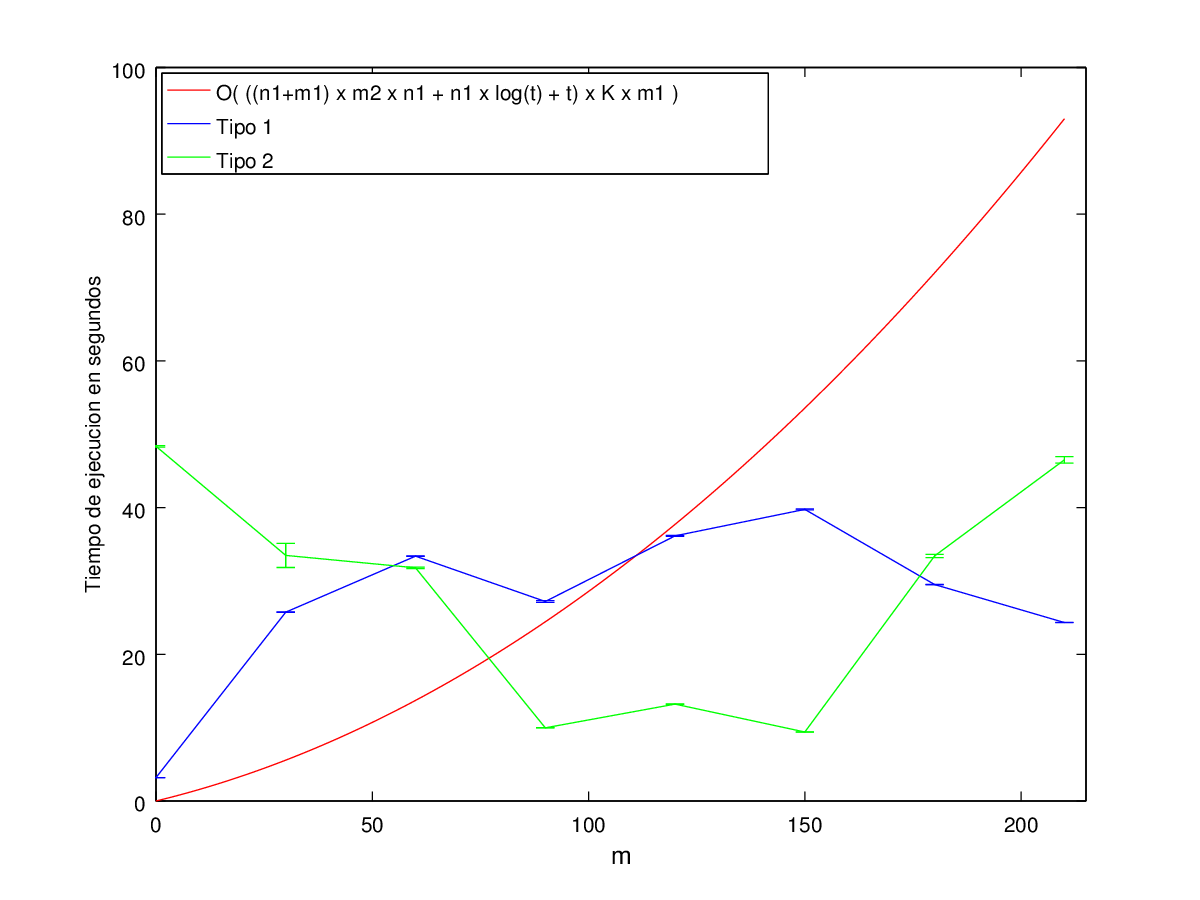
\includegraphics[height=10cm]{graficos/ejercicio6-exp1.png}
       \caption{Experimento 1}
	\end{figure}
\subsubsection*{Conclusiones}\;
        
        
        
\subsubsection*{Experimento 2}\;
\noindent Este experimento es similar al anterior, pero ahora se varía la cantidad de nodos. Para ello, para cada cantidad de nodos se definirá una función para determinar la cantidad de aristas que tendrá el grafo. \\
\noindent Se tuvieron en cuenta 4 funciones, con el fin de que el grafo obtenido no sea siempre uno especial y de esta forma poder analizar diferentes casos. 
        \begin{itemize}
        \item F1($n_1$) = $n_1$($n_1$-1))/2 = $m_1$ 
        \item F2($n_1$) = $n_1$-1 = $m_1$ 
        \item F3($n_1$) = 3$n_1$ = $m_1$ 
        \item F4($n_1$) = $n_1^{2}$/10 = $m_1$ 
		\end{itemize} 
Para generar los grafos con estas cantidades de aristas y nodos se utilizó el mismo generador que en el experimento anterior.
Este experimento se realizará de la misma manera utilizando primero la vecindad tipo 1 y luego la vecindad tipo 2.

\subsubsection*{Datos de entrada}\;
\noindent Los valores de $n_1$ tomados fueron desde $10$ hasta $30$ de $5$ en $5$. \\
       Los valores de $n_2$ y $m_2$ fueron $50$ y $30$ respectivamente. Estos valores fueron elegidos de forma arbitraria. Los valores de $cuantosVecinosMiro$, $tamanoMaximoListaTabu$ y $k$ fue $10$ para los $3$ parámetros.  Estos valores fueron elegidos de forma arbitraria. \\
        Para generar los grafos de forma aleatoria se utilizó el generador-grafo-rapido.cpp que se encuentra en la carpeta src y para correrlo se utilizó el exp2.sh que se encuentra en la carpeta exp/ejercicio6/exp2. \\
        Con el fin de acercarse a los valores reales y descartar posibles falsos resultados, se ejecuta la resolución del problema para cada una de los valores de $n_1$ cinco veces considerando luego el promedio entre los valores obtenidos pero graficando también el desvío estándar (la cantidad de repeticiones a realizar fue elegida arbitrariamente).\; 

\subsubsection*{Resultados}\;

    \begin{figure}[H]
      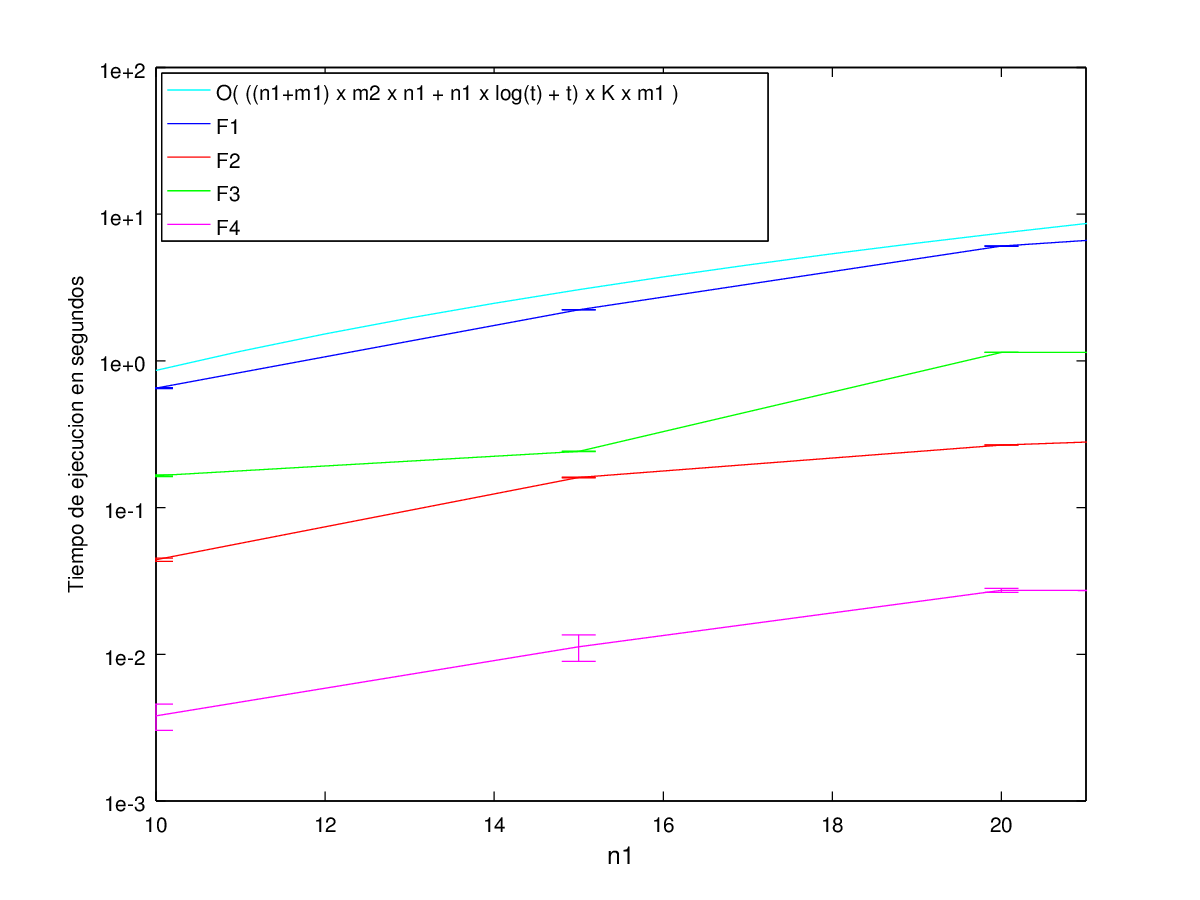
\includegraphics[height=10cm]{graficos/ejercicio6-exp2-tipo1.png}
       \caption{Experimento 2 - Vecindad tipo 1}
	\end{figure}

    \begin{figure}[H]
      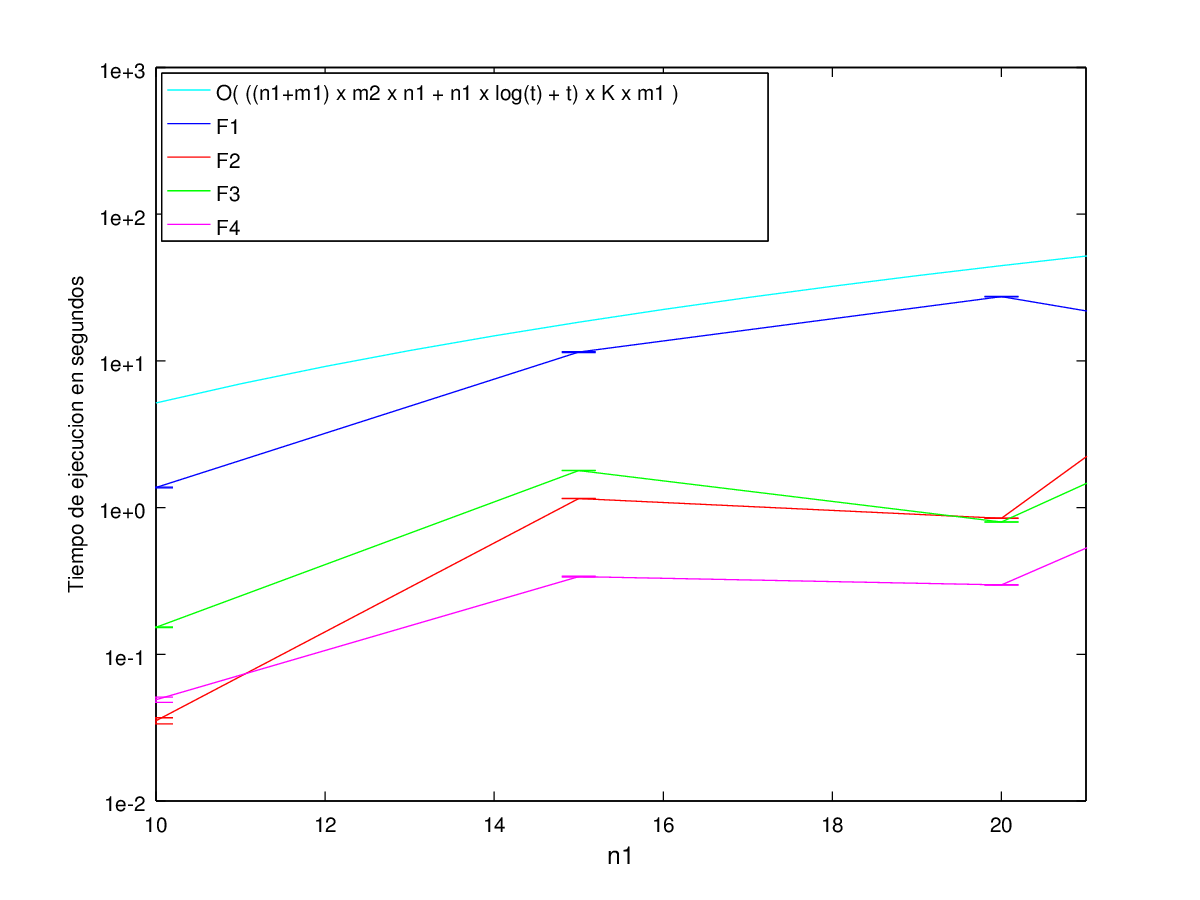
\includegraphics[height=10cm]{graficos/ejercicio6-exp2-tipo2.png}
       \caption{Experimento 2 - vecindad tipo 2}
	\end{figure}

\subsubsection*{Conclusiones}\;
Observamos que en todos los casos se respeta la complejidad propuesta(la curva de tiempo de computo se coloca por debajo de la de la cota de complejidad).\\
Se observa también comparando entre los 2 gráficos que el aplica vecindades del tipo 1 es considerablemente  mas rápido en todos los casos(en algunos mas que otros).Lo que nos lleva a concluir que el algoritmo de este tipo de vecindad se llega a ejecutar mas rápido, lo que no significa que sea el mejor pues para esto habría que analizar la calidad de las soluciones obtenidas(lo que haremos en un próximo experimento).\\ 
Adicionalmente se observa que el orden en que resultaron los tiempo de las distintas $F$ es el mismo en ambos grafos, lo que nos lleva a la conclusión de que los peores y mejores casos(al menos en cuanto a tiempo de computo) serán los mismos para ambos algoritmos.



\subsubsection*{Experimento 3}\; 
    El objetivo de este experimento fue extraer conclusiones acerca de la variación en el tiempo de cómputo requerido por el algoritmo para distintos valores de $m$ y $n$ variando los dos grafos al mismo tiempo pero siempre manteniendo $n_1$ igual a $n_2$ y $m_1$ igual a $m_2$. \\
Para generar los grafos con estas cantidades de aristas y nodos se utilizó el mismo generador que en el experimento anterior.
Este experimento se realizará utilizando primero la vecindad tipo 1 y luego la vecindad tipo 2.
        
\subsubsection*{Datos de entrada}\;
    \noindent Los valores de $n$ tomados fueron desde $10$ hasta $25$ de $5$ en $5$. Los valores de $cuantosVecinosMiro$, $tamanoMaximoListaTabu$ y $k$ fue $10$ para los $3$ parámetros. Estos valores fueron elegidos de forma arbitraria. \\
        Para generar los grafos de forma aleatoria se utilizó el generador-grafo-rapido.cpp que se encuentra en la carpeta src y para correrlo se utilizó el exp3.sh que se encuentra en la carpeta exp/ejercicio6/exp3. \\
        Con el fin de acercarse a los valores reales y descartar posibles falsos resultados, se ejecuta la resolución del problema para cada una de los valores de $n$ cinco veces considerando luego el promedio entre los valores obtenidos pero graficando también el desvío estándar (la cantidad de repeticiones a realizar fue elegida arbitrariamente).\; 

\subsubsection*{Resultados}\;

    \begin{figure}[H]
      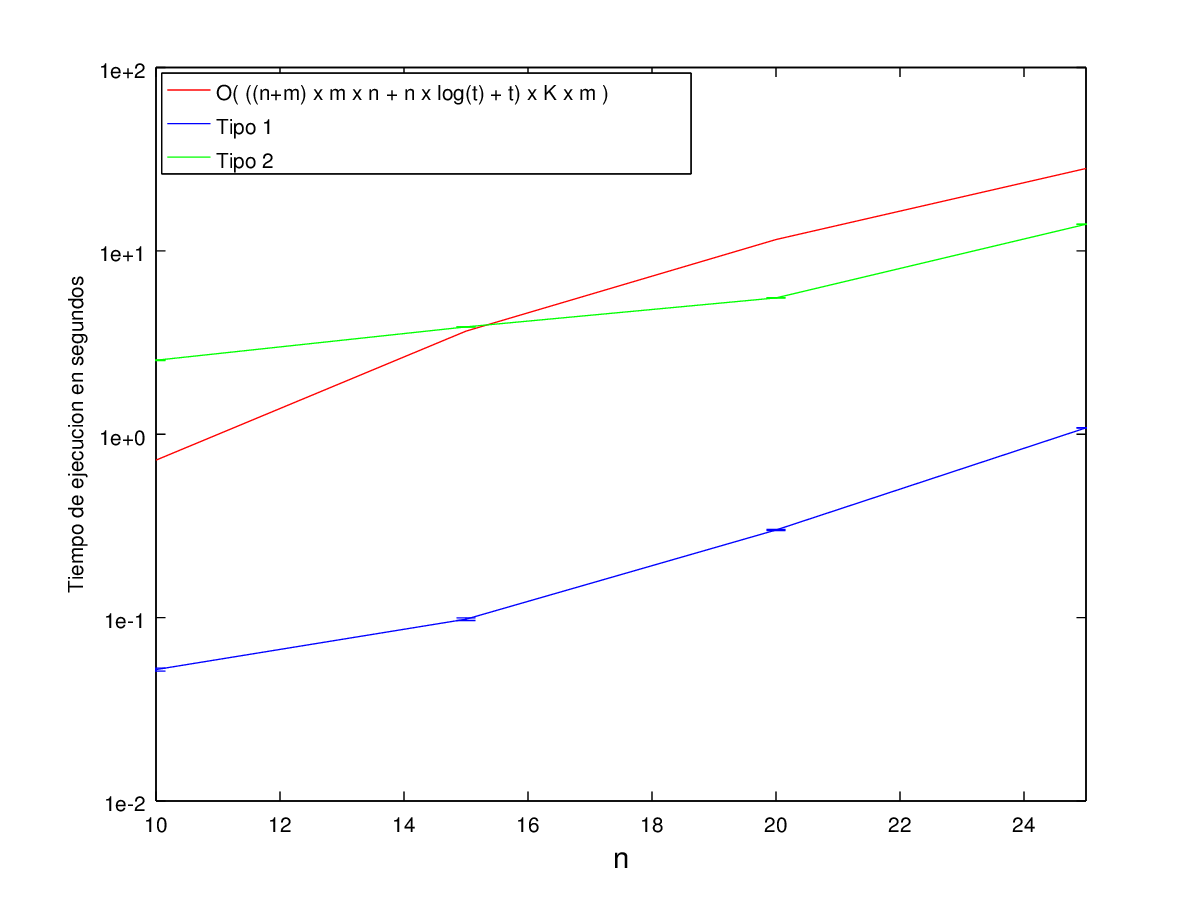
\includegraphics[height=10cm]{graficos/ejercicio6-exp3.png}
       \caption{Experimento 3}
	\end{figure}


\subsubsection*{Conclusiones}\;
Se observa en el gráfico, que ambos algoritmos parecen cumplir con la cota de complejidad asintótica propuesta, sin embargo, se puede ver también, como conjeturamos anteriormente, que el algoritmo de vecindades tipo 1 resulta ser mas eficiente que el de tipo 2, como ya dijimos esto no concluye que sea mejor pues sera necesario comparar primero la calidad de las soluciones, pero si podemos concluir que en cuanto al tiempo de ejecución es mejor el de vecindades tipo 1.


\subsubsection*{Experimento 4}\;
\noindent El objetivo de este experimento fue comparar los diferentes tipos de vecindades. Para ello se tomó en cuenta cuánto es el tiempo de cómputo y cuál es la cantidad de aristas que tiene el grafo solución para cada una de las vecindades. De esta forma, se logra analizar que vecindad es conveniente utilizar en determinados casos. Por ejemplo, en algunas ocasiones será beneficioso utilizar la vecindad que provea una respuesta en menor tiempo (aunque no sea la mejor) y en otras será ventajoso utilizar la vecindad que devuelva la solución más exacta posible, dándole más importancia a ésto que al tiempo que tarde en devolverla. \\
Para ello se utilizó el mismo generador que en el experimento 1.\\
Para realizar este experimento se ejecutaron las dos vecindades pasándoles por parámetro de entrada los mismos grafos, el mismo tamaño de la lista tabú, la misma cantidad de vecinos a tener en cuenta para cada iteración, y el mismo criterio de parada para poder realizar una comparación más exacta. 

\subsubsection*{Datos de entrada}\;
\noindent Los valores de $n_1$ tomados fueron desde $5$ hasta $20$ de $2$ en $2$. \\
       Los valores de $n_2$ y $m_2$ fueron $50$ y $200$ respectivamente. Los valores de $cuantosVecinosMiro$, $tamanoMaximoListaTabu$ y $k$ fue $10$ para los $3$ parámetros. Estos valores fueron elegidos de forma arbitraria. \\
        Para generar los grafos de forma aleatoria se utilizó el generador-grafo-rapido.cpp que se encuentra en la carpeta src y para correrlo se utilizó el exp4.sh que se encuentra en la carpeta exp/ejercicio6/exp4. \\
        Con el fin de acercarse a los valores reales y descartar posibles falsos resultados, se ejecuta la resolución del problema para cada una de los valores de $n_1$ cinco veces considerando luego el promedio entre los valores obtenidos pero graficando también el desvío estándar (la cantidad de repeticiones a realizar fue elegida arbitrariamente).\; 
\subsubsection*{Resultados}\;

    \begin{figure}[H]
      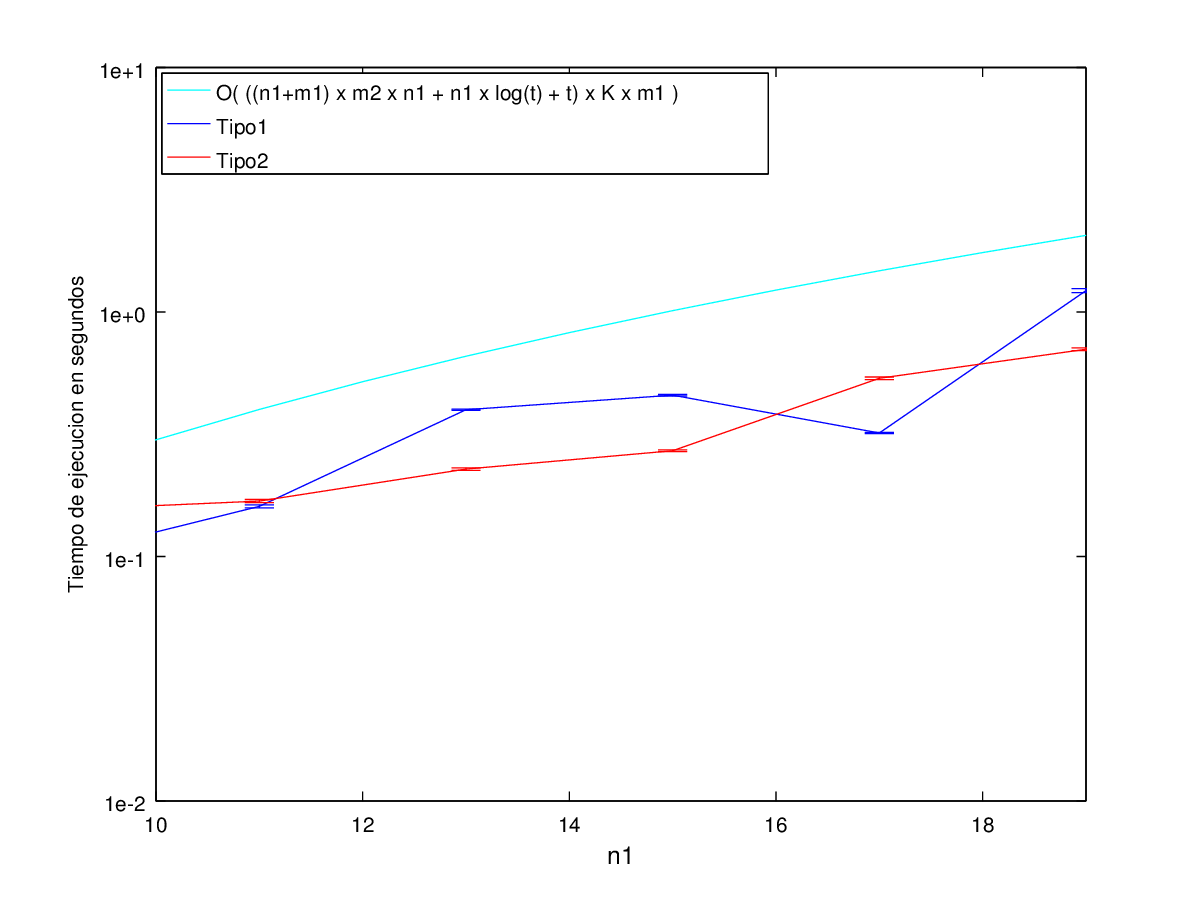
\includegraphics[height=10cm]{graficos/ejercicio6-exp4-tiempos.png}
       \caption{Experimento 4 - Comparando tiempos}
	\end{figure}

 \begin{figure}[H]
      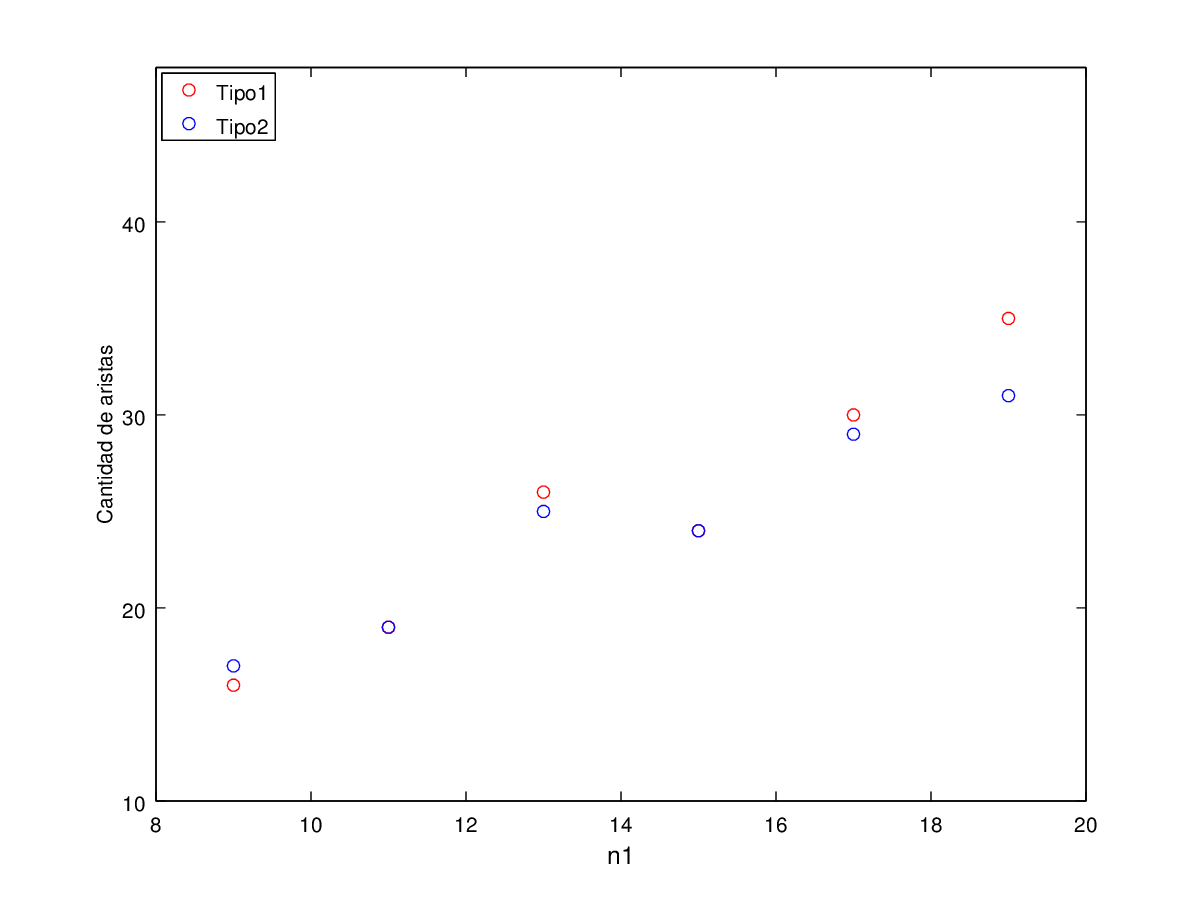
\includegraphics[height=10cm]{graficos/ejercicio6-exp4-aristas.png}
       \caption{Experimento 4 - Comparando cantidad de aristas}
	\end{figure}


\subsubsection*{Conclusiones}\;
En este Experimento el el gráfico de los tiempos, no se logra comprobar la conjetura de que el algoritmo con las vecindades tipo 1 es mas eficiente.\\
Se observa también del gráfico de los tiempos que ambos algoritmos se mantienen dentro del rango de complejidad esperada.\\
Finalmente, las conclusiones mas destacables de este experimento se pueden ver en el segundo gráfico, En este se ve como las soluciones brindadas por el algoritmo con las vecindades tipo 1 son superiores en todos los casos al de las vecindades tipo 2, en algunos casos se observa que la solución encontrada es considerablemente mejor(para la instancia de $n_1=20$), atribuimos a esta considerable diferencia el echo de que el algoritmo de tipo 1 resulto tardar mas para esta instancia que el de las vecindades tipo 2 a pesar de que experimentos pasados nos dieron el pie a conjeturar y concluir que las vecindades tipo 1 son también mas eficientes.\\
Concluimos entonces(con este experimento en conjunto con los anteriores):\\
El algoritmo de vecindades tipo 1 es considerablemente mejor en cuanto a la calidad de soluciones que provee.\\
El algoritmo de vecindades tipo 1 es mas eficiente excepto cuando encuentra una solución considerablemente mejor que la del algoritmo de vecindades tipo 2, en este caso podría resultar ligeramente mas lento.\\
Como conclusión general diremos que el algoritmo con las vecindades tipo 1 es mejor(para la gran mayoría de los casos).

\subsubsection*{Experimento 5}\;
\noindent En este experimento se buscará comparar cómo varía el tiempo de ejecución y la cantidad de aristas que tiene el grafo solución cuando se toman distintos tamaños máximos que puede tener la lista tabú. Para ello se dejarán constantes los grafos sobre los que se calcula el MCS, ambos generados de manera aleatoria, la cantidad de vecinos a tener en cuenta para cada iteración y el criterio de parada.\\
El generador utilizado será el mismo que en el experimento 1.\\
Se utilizará la vecindad que generó mejores resultados en el experimento anterior ya que el objetivo no es comparar entre vecindades si no comparar resultados cuando varía el tamaño de la lista tabú.

\subsubsection*{Datos de entrada}\;
\noindent Los valores de $tamanoMaximoListaTabu$ tomados fueron desde $5$ hasta $40$ de $5$ en $5$. \\
       Los valores de $n_1$ y $m_1$ fueron $50$ y $200$ respectivamente, al igual que $n_2$ y $m_2$ ($n_1 = n_2$ y $m_1 = m_2$). Los valores de $cuantosVecinosMiro$, y $k$ fue $10$ para los $2$ parámetros. Estos valores fueron elegidos de forma arbitraria. \\
        Para generar los grafos de forma aleatoria se utilizó el generador-grafo-rapido.cpp que se encuentra en la carpeta src y para correrlo se utilizó el exp5.sh que se encuentra en la carpeta exp/ejercicio6/exp5. \\
        Con el fin de acercarse a los valores reales y descartar posibles falsos resultados, se ejecuta la resolución del problema para cada una de los valores de $tamanoMaximoListaTabu$ cinco veces considerando luego el promedio entre los valores obtenidos pero graficando también el desvío estándar (la cantidad de repeticiones a realizar fue elegida arbitrariamente).\; 

\subsubsection*{Resultados}\;
    \begin{figure}[H]
      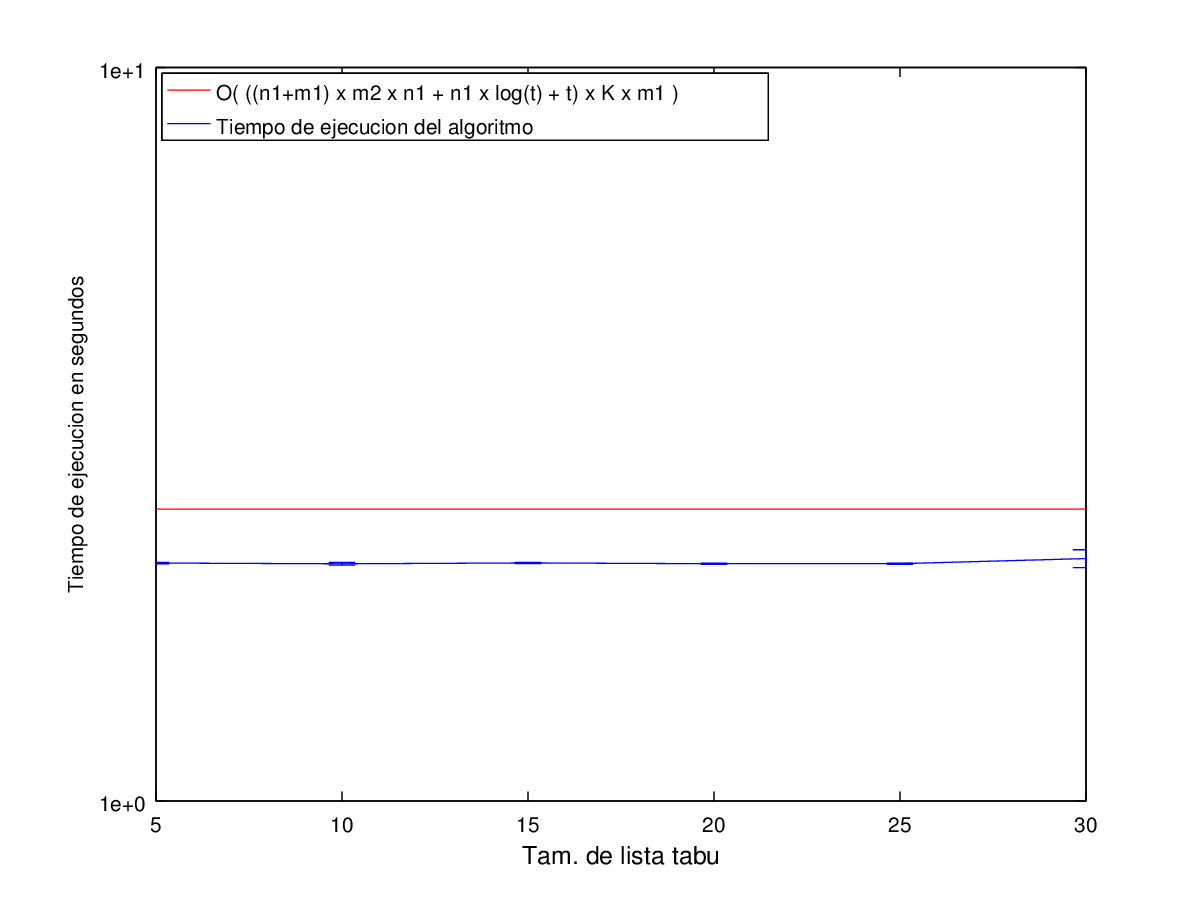
\includegraphics[height=10cm]{graficos/ejercicio6-exp5-tiempos.png}
       \caption{Experimento 5 - Comparando tiempos}
	\end{figure}

 \begin{figure}[H]
      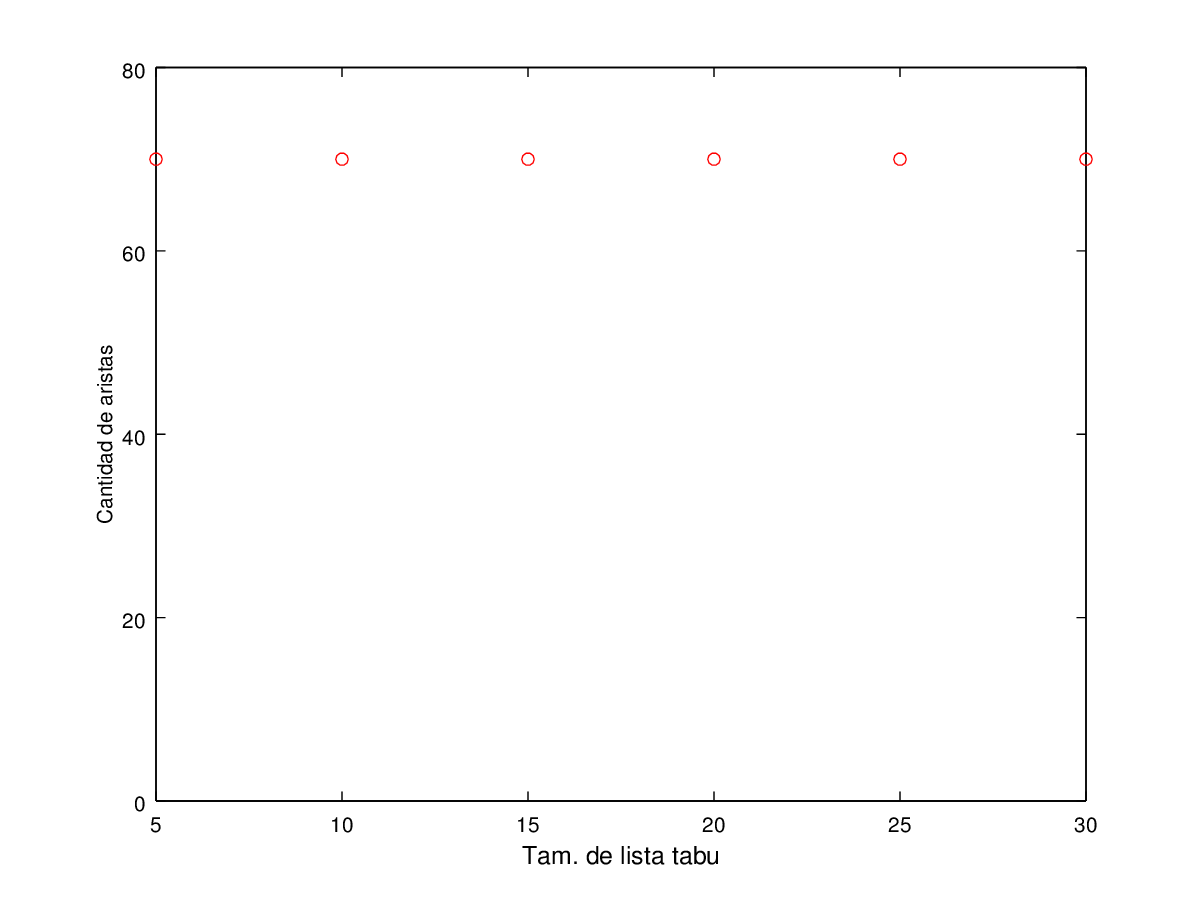
\includegraphics[height=10cm]{graficos/ejercicio6-exp5-aristas.png}
       \caption{Experimento 5 - Comparando cantidad de aristas}
	\end{figure}


\subsubsection*{Conclusiones}\;
Se observa que el tiempo de ejecución se mantiene constante a pesar del cambio en el tamaño de la lista tabú.Esto, conjeturamos, resulta así dado que:\\
-El tiempo de creación de la lista tabú, es irrelevante para el tiempo del problema, es decir el tiempo de crear la lista de t posiciones es despreciable en comparación al Tiempo que llevan las comparaciones de vecindades sucesivas.\\
-La lista tabú no parece llenarse siempre, es decir que por mas grande que se haga esta lista, solo se usa una parte reducida de esta, las búsquedas al ser logarítmicas en el tamaño de elementos tabú (multiplicado por $n_1$), puede despreciarse también en relación al resto del algoritmo ya que los ordenes de complejidad del resto de las operaciones son significativamente mas altos.\\ Incluso para n y m fijos,como es el caso hacer variar el t ligeramente, como esta echo, no parece contribuir significativamente, probablemente se deba a que el uso de la lista tabú es reducido.\\
Ademas cabe recalcar que la complejidad propuesta esta calculada en el caso del peor escenario posible, el cual es difícil de replicar y es poco probable que se re replique en un caso aleatorio(esto esta explicado en el desarrollo de complejidad).\\
Concluimos entonces que la gran mayoría de los casos el tamaño de la lista tabú no es un factor influyente en la cantidad de aristas ni en el tiempo de computo(a pesar de aparecer en la complejidad del peor caso, este peor caso es un caso excepcional y poco común).
 
\subsubsection*{Experimento 6}\;
\noindent En este experimento se buscará comparar cómo varía el tiempo de ejecución y la cantidad de aristas que tiene el grafo solución cuando se toman distintas cantidades de vecinos a tomar en cuenta para cada iteración. Para ello se dejarán constantes los grafos sobre los que se calcula el MCS, ambos generados de manera aleatoria, el tamaño máximo que puede tomar la lista tabú y el criterio de parada.\\
El generador utilizado será el mismo que en el experimento 1.\\
Se utilizará la vecindad que generó mejores resultados en los primeros experimentos ya que el objetivo no es comparar entre vecindades si no comparar resultados cuando varían las cantidades de vecinos a tomar en cuenta para cada iteración.

\subsubsection*{Datos de entrada}\;
\noindent Los valores de $cuantosVecinosMiro$ tomados fueron desde $5$ hasta $30$ de $5$ en $5$. \\
       Los valores de $n_1$ y $m_1$ fueron $50$ y $200$ respectivamente, al igual que $n_2$ y $m_2$ ($n_1 = n_2$ y $m_1 = m_2$). El valor de $tamanoMaximoListaTabu$ fue $20$ y $k$ fue $10$. Estos valores fueron elegidos de forma arbitraria. \\
        Para generar los grafos de forma aleatoria se utilizó el generador-grafo-rapido.cpp que se encuentra en la carpeta src y para correrlo se utilizó el exp6.sh que se encuentra en la carpeta exp/ejercicio6/exp6. \\
        Con el fin de acercarse a los valores reales y descartar posibles falsos resultados, se ejecuta la resolución del problema para cada una de los valores de $cuantosVecinosMiro$ cinco veces considerando luego el promedio entre los valores obtenidos pero graficando también el desvío estándar (la cantidad de repeticiones a realizar fue elegida arbitrariamente).\; 
        
\subsubsection*{Resultados}\;
    \begin{figure}[H]
      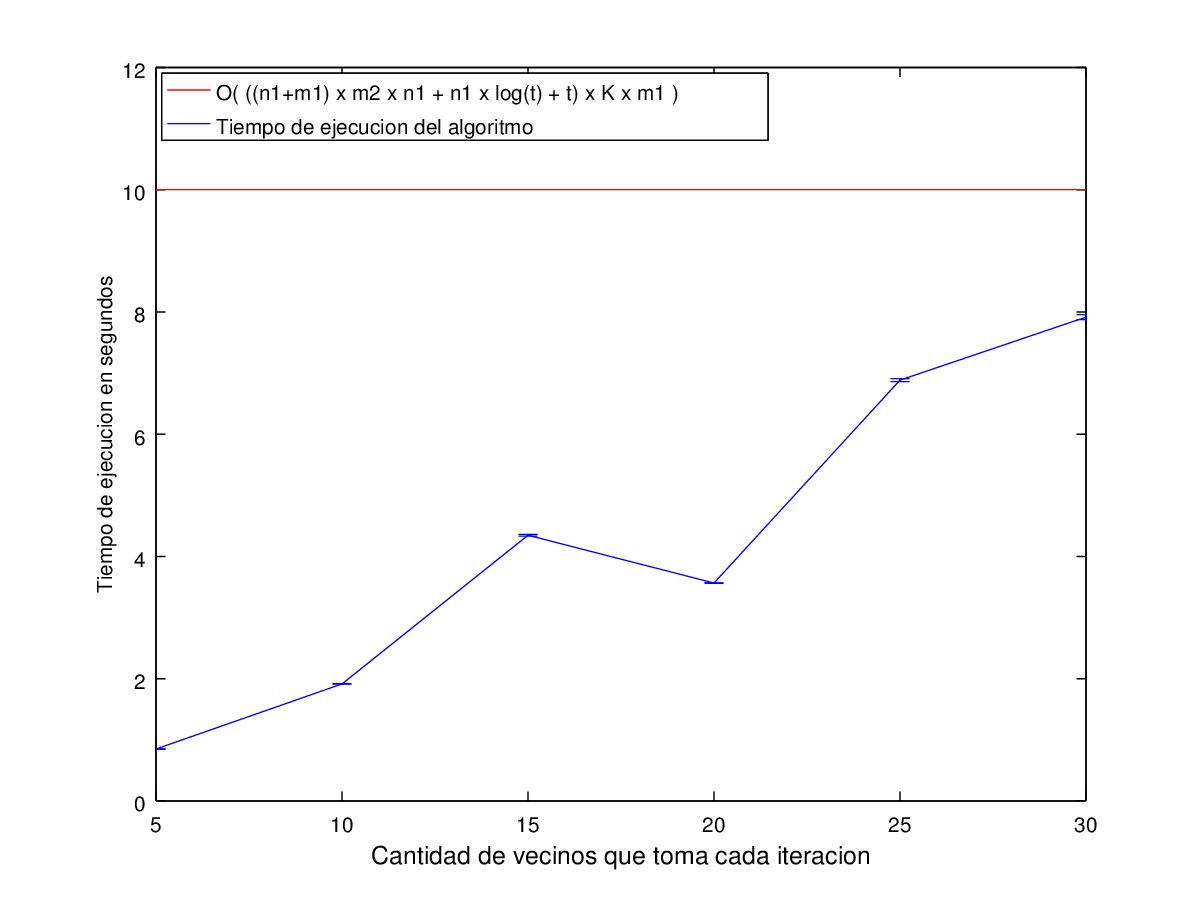
\includegraphics[height=10cm]{graficos/ejercicio6-exp6-tiempos.png}
       \caption{Experimento 6 - Comparando tiempos}
	\end{figure}

 \begin{figure}[H]
      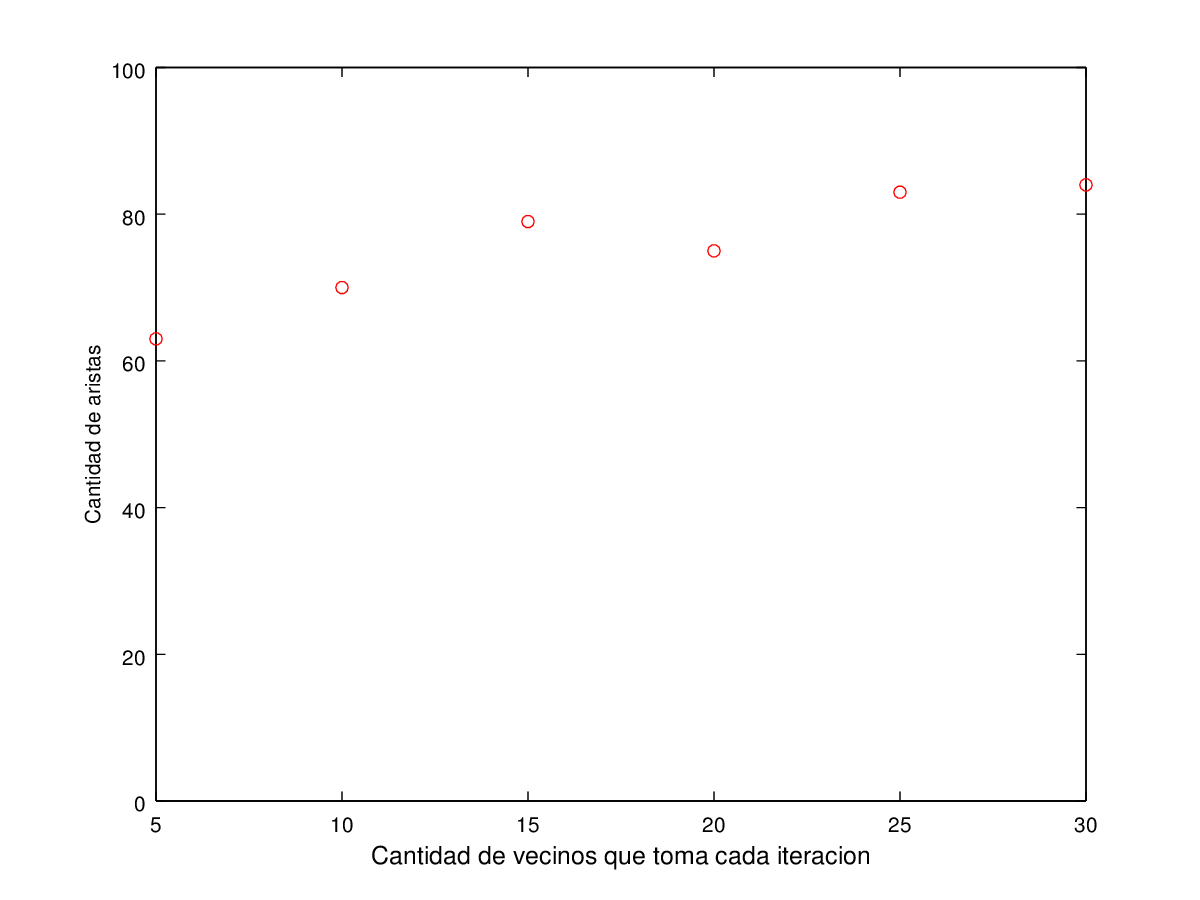
\includegraphics[height=10cm]{graficos/ejercicio6-exp6-aristas.png}
       \caption{Experimento 6 - Comparando cantidad de aristas}
	\end{figure}


\subsubsection*{Conclusiones}\;
En el primer gráfico (el de tiempos) se observa como influye de manera cuasi-linear la cantidad de vecinos a tomar en cada iteración hasta llegar al limite de $n_1$ vecinos , que es el tamaño de toda la vecindad(es por esto que la linea de cota es una constante) esta constante da la cota en caso que la cantidad de vecinos a tomar sea $n_1$ osea toda la vecindad, como el resto de los parámetros se mantienen constantes la cota sera constante.\\
En el segundo gráfico apreciamos que la diferencia entre cantidad de vecinos a tomar variara la cantidad de aristas en la solución(hay un incremento de aproximadamente un 25\%, solo variando la cantidad de vecinos a tomar).\\
Concluimos entonces que reducir el numero de vecinos a tener en cuenta puede ser útil para reducir el tiempo de computo (se reduce linealmente el tiempo) especialmente en los casos que $n_1$ es relativamente grande(recordamos que $n_1$, hace referencia a la cantidad de nodos del grafo mas chico),En cambio si alguno de los 2 grafos es relativamente chico sera aconsejable que la cantidad de vecinos que se toman en cuenta sea alta(cuanto mas cercano a $n_1$ mejor) pues en este caso no afectara mucho al tiempo de computo y puede mejorar la solución considerablemente.\\
Por otra parte incluso en grafos de gran cantidad de nodos($n_1$ grande) puede ser positivo establecer una cantidad de vecinos a considerar alta ya que es altamente probable que mejore la solución considerablemente, aunque en contraposición si se notara un incremento en el tiempo de computo.


\subsubsection*{Experimento 7}\;
\noindent En este experimento se buscará comparar cómo varía el tiempo de ejecución cuando varía la cantidad de iteraciones que deben pasar sin obtener una solución mejor a la que se tiene hasta el momento y termine de ejecutar el algoritmo(el criterio de parada,el  K). Para ello se dejan constantes los grafos sobre los que se calcula el MCS, ambos generados de manera aleatoria, el tamaño máximo que puede tomar la lista tabú y la cantidad de vecinos a tomar en cuenta para cada iteración.\\
El generador utilizado será el mismo que en el experimento 1.\\
Se utilizará la vecindad que generó mejores resultados en los primeros experimentos ya que el objetivo no es comparar entre vecindades si no comparar resultados cuando varía la cantidad de iteraciones que deben pasar sin obtener una solución mejor a la que se tiene hasta el momento y termine de ejecutar el algoritmo.

\subsubsection*{Datos de entrada}\;
\noindent Los valores de $k$ tomados fueron desde $5$ hasta $25$ de $5$ en $5$. \\
       El valor de $n_1$ fue $1000$ y el de $n_2$ fue $150$. El de $m_1$ fue $200$ al igual que $m_2$.  Los valores de $cuantosVecinosMiro$ y $tamanoMaximoListaTabu$ fue $20$ para los $2$ parámetros. Estos valores fueron elegidos de forma arbitraria. \\
        Para generar los grafos de forma aleatoria se utilizó el generador-grafo-rapido.cpp que se encuentra en la carpeta src y para correrlo se utilizó el exp7.sh que se encuentra en la carpeta exp/ejercicio6/exp7. \\
        Con el fin de acercarse a los valores reales y descartar posibles falsos resultados, se ejecuta la resolución del problema para cada una de los valores de $k$ cinco veces considerando luego el promedio entre los valores obtenidos pero graficando también el desvío estándar (la cantidad de repeticiones a realizar fue elegida arbitrariamente).\;
\subsubsection*{Resultados}\;
    \begin{figure}[H]
      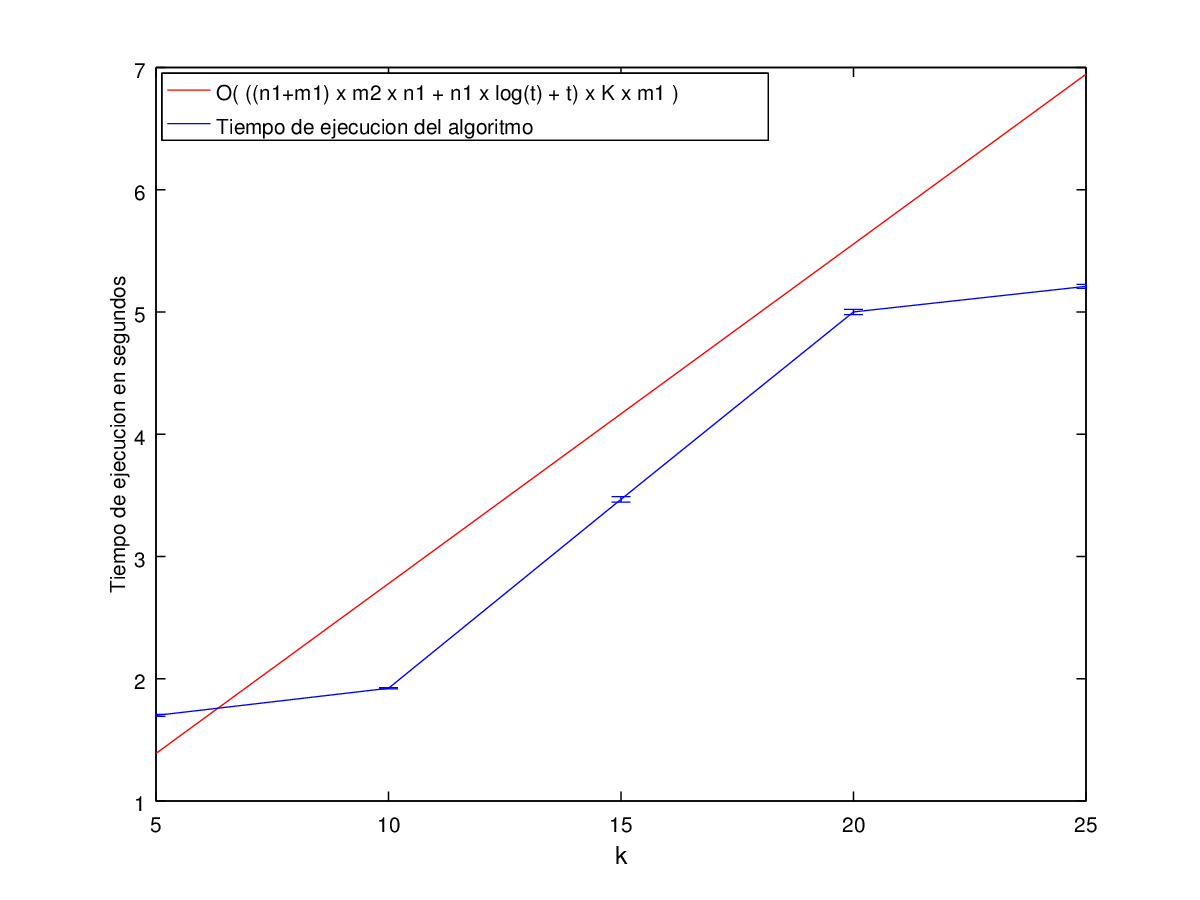
\includegraphics[height=10cm]{graficos/ejercicio6-exp7-tiempos.png}
       \caption{Experimento 7 - Comparando tiempos}
	\end{figure}



\subsubsection*{Conclusiones}\;
Se observa como era esperado el comportamiento aproximadamente lineal en $k$(el limite, criterio de parada o cantidad de veces que continua el algoritmo sin encontrar nada mejor).\\
Concluimos de este experimento que el aumento del criterio de parada aumenta el tiempo de computo linealmente aunque aumentarlo puede eventualmente llevar a una mejor solución.

